\documentclass[a4paper]{article}
\usepackage{ctex}
\usepackage{amsmath, amssymb, amsthm}
\usepackage{moreenum}
\usepackage{mathtools}
\usepackage{url}
\usepackage{bm}
\usepackage{enumitem}
\usepackage{graphicx}
\usepackage{listings}
\usepackage{color}

\usepackage{fontspec}
\usepackage{xcolor}

\usepackage{float}

\definecolor{codekeyword}{RGB}{171, 0, 216}
\definecolor{codetypename}{RGB}{29, 37, 251}
\definecolor{codevariable}{RGB}{10, 23, 126}
\definecolor{codestring}{RGB}{157, 0, 25}
\definecolor{codecomment}{RGB}{31, 129, 19}
\definecolor{codebackground}{RGB}{230 235 245}

\newfontfamily\cascadia[Ligatures=ResetAll]{Cascadia Code}

\lstset{
    basicstyle          =   \footnotesize\cascadia,          % 基本代码风格
    keywordstyle        =   \bfseries,          % 关键字风格
    commentstyle        =   \rmfamily\itshape,  % 注释的风格,斜体
    stringstyle         =   \ttfamily,  % 字符串风格
    flexiblecolumns,                % 别问为什么,加上这个
    numbers             =   left,   % 行号的位置在左边
    showspaces          =   false,  % 是否显示空格,显示了有点乱,所以不现实了
    numberstyle         =   \cascadia,    % 行号的样式,小五号,tt等宽字体
    showstringspaces    =   false,
    captionpos          =   t,      % 这段代码的名字所呈现的位置,t指的是top上面
    backgroundcolor     =   \color{codebackground},
    breaklines          =   true,
    frame               =   l,
}

\lstdefinestyle{Python}{
    language        =   Python, % 语言选Python
    basicstyle      =   \zihao{-5}\ttfamily,
    numberstyle     =   \zihao{-5}\ttfamily,
    keywordstyle    =   \color{blue},
    keywordstyle    =   [2] \color{teal},
    stringstyle     =   \color{magenta},
    commentstyle    =   \color{red}\ttfamily,
    breaklines      =   true,   % 自动换行,建议不要写太长的行
    columns         =   fixed,  % 如果不加这一句,字间距就不固定,很丑,必须加
    basewidth       =   0.5em,
}
\usepackage{subcaption}
\usepackage{booktabs} % toprule
\usepackage[mathcal]{eucal}
\usepackage[thehwcnt = 2]{iidef}

\usepackage{pdfpages}

\setenumerate[1]{label=(\arabic{*})}
\setenumerate[2]{label=\arabic{*})}


\thecourseinstitute{清华大学电子工程系}
\thecoursename{\textbf{媒体与认知}}
\theterm{2023-2024学年春季学期}
\hwname{作业}
\begin{document}
\courseheader
\name{毕嘉仪}
\vspace{3mm}
\centerline{\textbf{\Large{理论部分}}}

\section{单选题(15分)}
\subsection{\underline{D}}

\subsection{\underline{A}}

\subsection{\underline{A}}

\subsection{\underline{C}}

\subsection{\underline{B}}

\section{计算题(15 分)}
% 计算题1
\subsection{隐含马尔可夫模型}

\hspace{2em}暑假中,小E每天进行一项体育活动,包括跑步(R)、游泳(S)和打球(B),所选择的体育活动受某种潜在因素(如心情)的影响。小E每天把进行体育活动的照片发至微信朋友圈,我们可以根据观测信息推测该潜在因素的状态。

\hspace{2em}假设该潜在因素分为$S_1$和$S_2$两种状态。在$S_1$时,小E选择三种体育活动的概率分别为0.6,0.2,0.2;在$S_2$时,小E选择三种体育活动的概率分别为0.1,0.6,0.3。

\hspace{2em}该潜在因素的变化也有一定规律,若某天处于$S_1$的状态,第二天处于$S_1$和$S_2$的状态的概率分别为0.5,0.5;若某天处于$S_2$的状态,第二天处于$S_1$和$S_2$的状态的概率分别为0.6,0.4。

\hspace{2em}暑假第一天处于$S_1$和$S_2$的状态的概率均为0.5。

\vspace{3mm}
(1) 采用隐含马尔可夫模型(HMM)对小E暑假体育活动安排进行建模,{\color{blue}请写出HMM对应的参数$\lambda=\{\pi, A, B\}$}。

\begin{proof}[解]
    有题意可知,初始概率分布为
    \[\pi = \begin{bmatrix}
        0.5\\0.5
    \end{bmatrix}\]

    概率转移矩阵为
    \[A = \begin{bmatrix}
        0.5 & 0.5\\
        0.6 & 0.4\\
    \end{bmatrix}\]

    观测结果概率矩阵为
    \[B = \begin{bmatrix}
        0.6 & 0.2 & 0.2\\
        0.1 & 0.6 & 0.3
    \end{bmatrix}\]
\end{proof}

(2) 假设暑假第1、2、3天小E所进行的体育活动依次为跑步(R)、打球(B)和游泳(S),{\color{blue}请计算出现该观测序列的概率}。
\begin{proof}[解]
    利用前向算法:
    \begin{align*}
        \alpha_1(S_1) & = \pi_1 B_{11} = 0.5 \times 0.6 = 0.3\\
        \alpha_1(S_2) & = \pi_2 B_{21} = 0.5 \times 0.1 = 0.05\\
        \alpha_2(S_1) & = (\alpha_1(S_1) A_{11} + \alpha_1(S_2) A_{21}) B_{13}\\
        & = (0.3 \times 0.5 + 0.05 \times 0.6) \times 0.2 = 0.036 \\
        \alpha_2(S_2) & = (\alpha_1(S_1) A_{12} + \alpha_1(S_2) A_{22}) B_{23} \\
        & = (0.3 \times 0.5 + 0.05 \times 0.4) \times 0.3 = 0.051\\
        \alpha_3(S_1) & = (\alpha_2(S_1) A_{11} + \alpha_2(S_2) A_{21}) B_{12} \\
        & = (0.036 \times 0.5 + 0.051 \times 0.6) \times 0.2 = 0.00972\\
        \alpha_3(S_2) & = (\alpha_2(S_1) A_{12} + \alpha_2(S_2) A_{22})B_{22} \\
        & = (0.036 \times 0.5 + 0.051 \times 0.4) \times 0.6 = 0.02304\\
        \therefore P(O \mid \lambda) & = \alpha_3(S_1) + \alpha_3(S_2) = 0.03276
    \end{align*}
\end{proof}

(3) 在(2)的条件下。{\color{blue}请利用Viterbi算法推测暑假第1、2、3天最可能的隐含状态序列}。
\begin{proof}[解]
    由Viterbi算法:
    \begin{align*}
        \delta_1(1) & = \pi_1 B_{11} = 0.3 \\
        \delta_1(2) & = \pi_2 B_{21} = 0.05 \\
        \varphi_1(1) & = \varphi_1(2) = 0 \\
        \\
        \delta_2(1) & = \max\{\delta_1(1)A_{11}, \delta_1(2)A_{12}\}B_{13} \\
            & = \max\{0.3 \times 0.5, 0.05 \times 0.5\} \times 0.2 = 0.03 \\
        \delta_2(2) & = \max\{\delta_1(1)A_{21}, \delta_1(2)A_{22}\}B_{23} \\
            & = \max\{0.3 \times 0.6, 0.05 \times 0.4\} \times 0.3 = 0.054 \\
        \varphi_2(1) & = \arg \max\{\delta_1(1)A_{11}, \delta_1(2)A_{12}\} \\
            & = \arg \max\{0.3 \times 0.5, 0.05 \times 0.5\} = 1 \\
        \varphi_2(2) & = \arg \max\{\delta_1(1)A_{21}, \delta_1(2)A_{22}\} \\
            & = \arg \max\{0.3 \times 0.6, 0.05 \times 0.4\} = 1 \\
        \\
        \delta_3(1) & = \max\{\delta_2(1)A_{11}, \delta_2(2)A_{12}\}B_{12} \\
            & = \max\{0.03 \times 0.5, 0.054 \times 0.5\} \times 0.2 = 0.0054 \\
        \delta_3(2) & = \max\{\delta_2(1)A_{21}, \delta_2(2)A_{22}\}B_{22} \\
            & = \max\{0.03 \times 0.6, 0.054 \times 0.4\} \times 0.6 = 0.01296 \\
        \varphi_3(1) & = \arg \max\{\delta_2(1)A_{11}, \delta_2(2)A_{12}\} \\
            & = \arg \max\{0.03 \times 0.5, 0.054 \times 0.5\} = 2 \\
        \varphi_3(2) & = \arg \max\{\delta_2(1)A_{21}, \delta_2(2)A_{22}\} \\
            & = \arg \max\{0.03 \times 0.6, 0.054 \times 0.4\} = 2 \\
        \\
        q_3^* & = \arg \max\{\delta_3(1), \delta_3(2)\} = \arg\max\{0.0054, 0.01296\} = 1 \\
        q_2^* & = \varphi_3(q_3^*) = \varphi_3(1) = 2 \\
        q_1^* & = \varphi_2(q_2^*) = \varphi_2(2) = 1 \\
        \therefore O^* & = \{1, 2, 1\} \\
    \end{align*}
\end{proof}


% 请根据是否选择自选课题的情况选择“编程作业报告”或“自选课题开题报告”中的一项完成
\section{编程作业报告}
\subsection{模型的训练与测试}
\begin{enumerate}
    \item 数据预处理与模型训练
    
    输入:
    \lstinputlisting{../file/1-1-in.txt}

    输出:验证集上loss和perplexity的变化:
    \begin{figure}[H]
        \centering
        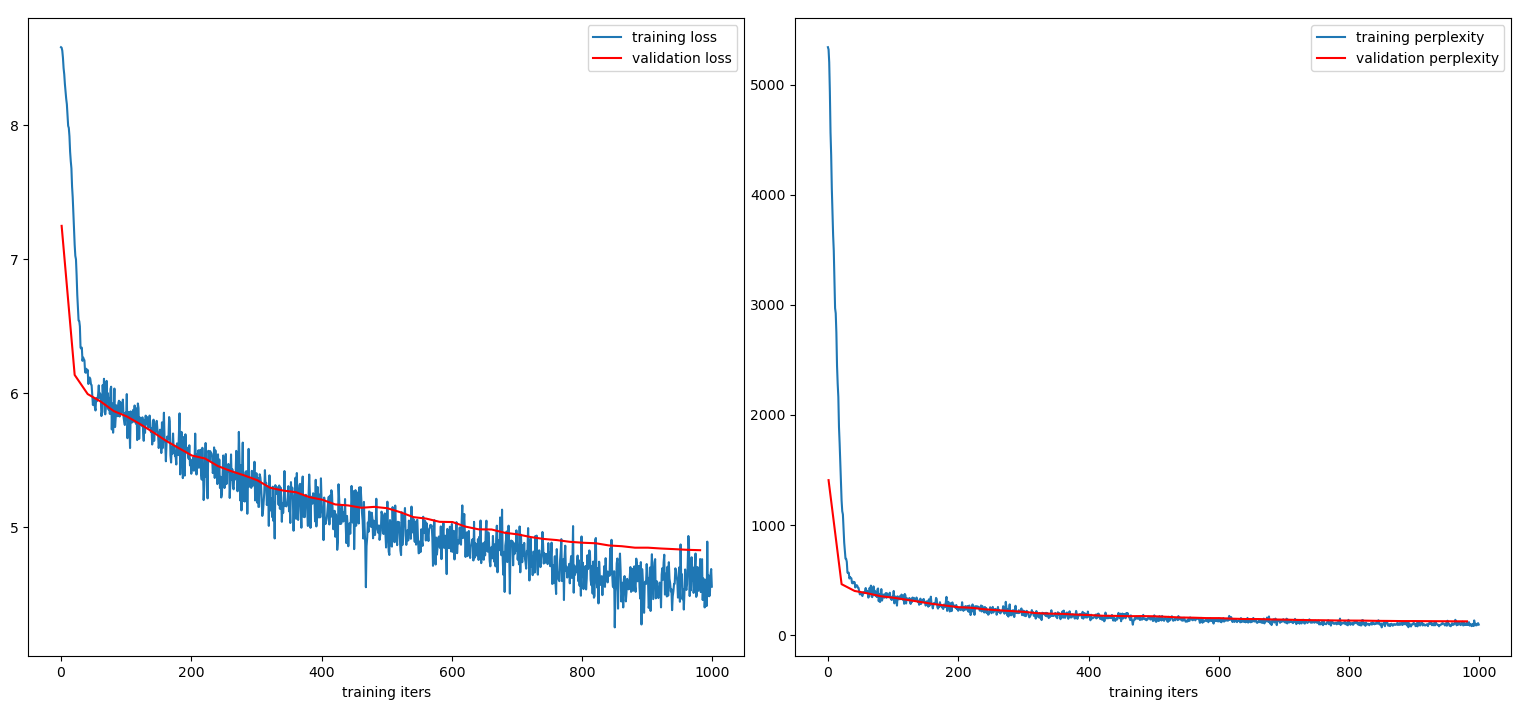
\includegraphics[width=0.9\linewidth]{../img/1.png}
    \end{figure}


    \item 模型文本生成结果
    
    \begin{enumerate}
        \item 默认配置以及指定生成文本
        
        分别输入:
        \lstinputlisting{../file/1-2-in.txt}

        输出分别为:
        \lstinputlisting{../file/1-2-out.txt}

        \item 生成质量较好的
        
        \begin{lstlisting}
+++卜算子(次韵)
满梦断云偏如去。一夜月十百般诗,犹有长凄凉。
望横台,当时疏影,休休留得。一枝一枕中却寻,看花满地。
        \end{lstlisting}

        \item 生成质量较差的
        
        \begin{lstlisting}
+++浣溪沙(送旅)
花容事古平。闲恋山明千古秋光。空光明夜行秋风雨语,花影边青桃花。
旧事何须能无计,愁情犹是留春又。春衫著情情情情。
        \end{lstlisting}
    \end{enumerate}
\end{enumerate}

\subsection{探究位置编码和残差连接在模型中的作用}
\begin{enumerate}
    \item 关闭位置编码
    
    分别输入:
    \lstinputlisting{../file/2-1-in.txt}

    结果:
    \begin{figure}[H]
        \centering
        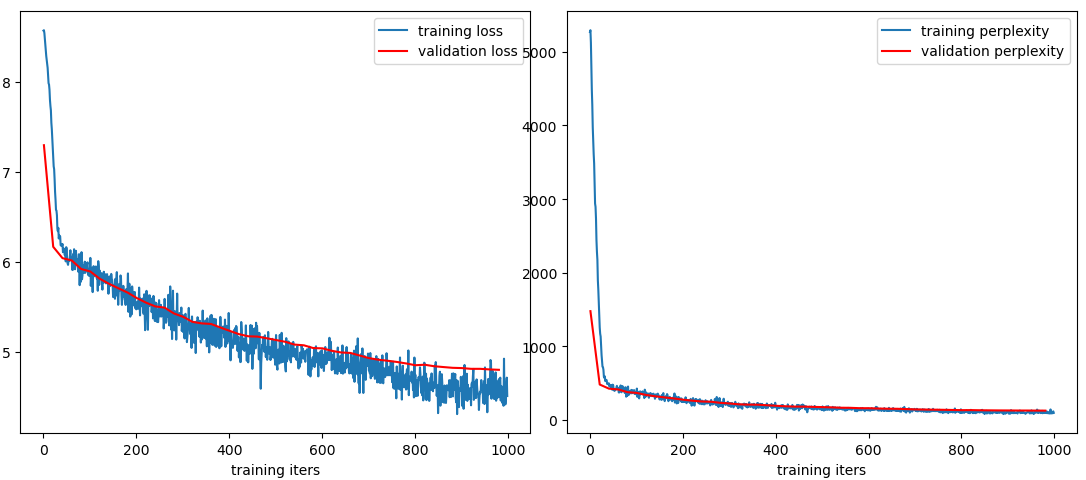
\includegraphics[width=0.8\linewidth]{../img/2-1.png}
    \end{figure}

    \lstinputlisting{../file/2-1-out.txt}
    
    \item 关闭残差连接的训练与测试命令
    
    分别输入:
    \lstinputlisting{../file/2-2-in.txt}

    结果:
    \begin{figure}[H]
        \centering
        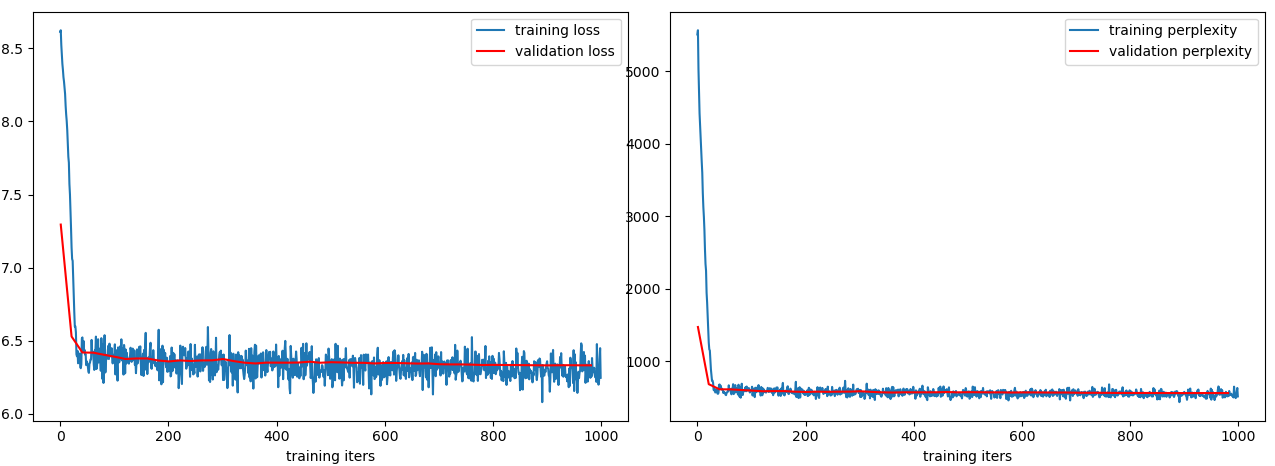
\includegraphics[width=0.8\linewidth]{../img/2-2.png}
    \end{figure}

    \lstinputlisting{../file/2-2-out.txt}
\end{enumerate}

可以看到验证集上loss和perplexity都高于默认配置且下降速率缓慢,生成结果也都远不如默认配置下的生成结果,no\_res模型甚至出现了严重胡言乱语行为。

\subsection{可视化}
可视化结果:
\begin{figure}[H]
    \centering
        \begin{subfigure}[b]{.45\linewidth}
            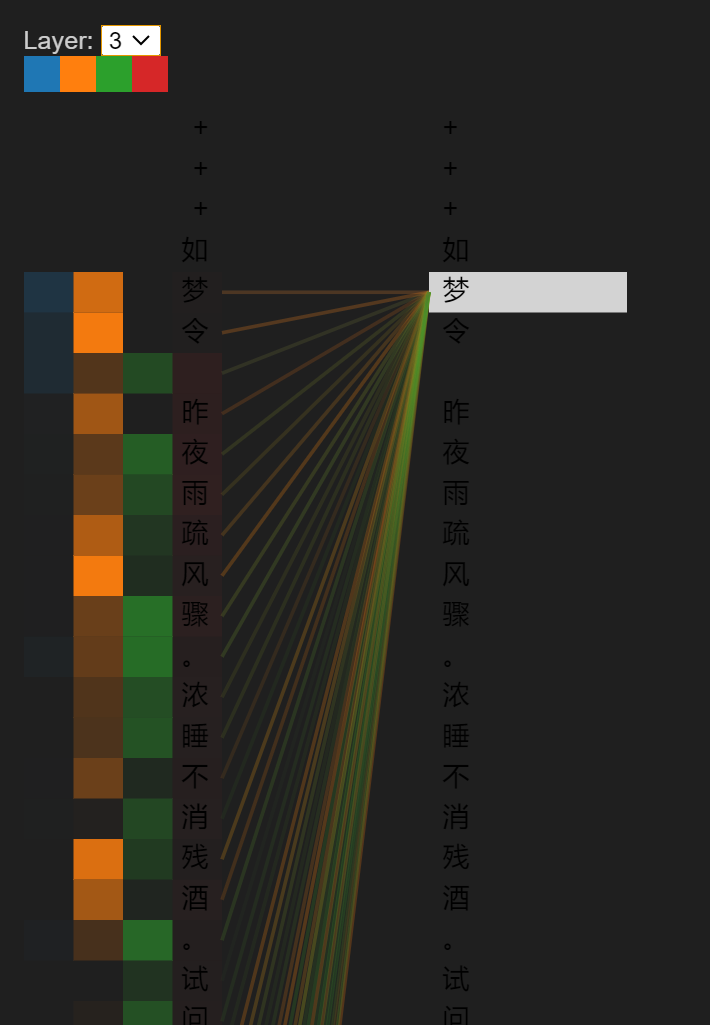
\includegraphics[width=\linewidth]{../img/3-1.png}
        \end{subfigure}
        \begin{subfigure}[b]{.5\linewidth}
            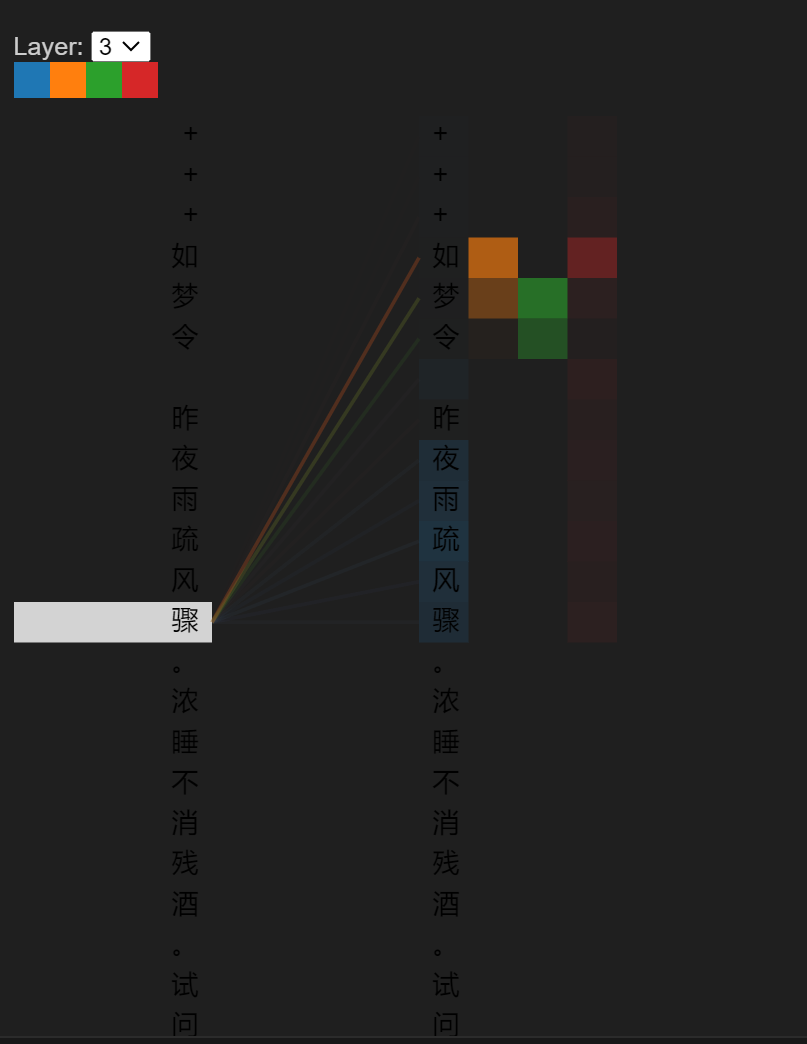
\includegraphics[width=\linewidth]{../img/3-2.png}
        \end{subfigure}
\end{figure}

许多的字的注意力系数在词牌上都达到较大值,可以看到模型主要是关联了词牌名与词面内容而进行生成,而没有针对词牌的格式与声韵或者句内逻辑进行联想。

\end{document}



%%% Local Variables:
%%% mode: late\rvx
%%% TeX-master: t
%%% End:
